\documentclass[border=3mm]{standalone}
\usepackage{tikz}
\usepackage{mathptmx}
\usetikzlibrary{arrows.meta,calc}

\begin{document}
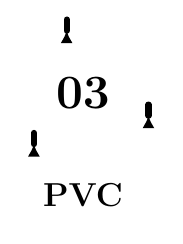
\begin{tikzpicture}[line cap=round, line join=round]
    % Tam giác tái chế 3 mũi tên
    % 3 góc ở 90 độ, 210 độ, 330 độ
    \def\R{1.2}
    \coordinate (A) at (90:\R);
    \coordinate (B) at (210:\R);
    \coordinate (C) at (330:\R);
    
    % Vẽ 3 nhánh mũi tên bo góc
    \draw[line width=2.2pt, -{Latex[length=4.5pt, width=4.5pt]}] 
        ($(A)!0.2!(B)$) -- ($(B)!0.8!(A)$);
    \draw[line width=2.2pt, -{Latex[length=4.5pt, width=4.5pt]}] 
        ($(B)!0.2!(C)$) -- ($(C)!0.8!(B)$);
    \draw[line width=2.2pt, -{Latex[length=4.5pt, width=4.5pt]}] 
        ($(C)!0.2!(A)$) -- ($(A)!0.8!(C)$);
        
    % Số 03 ở giữa
    \node at (0, 0.05) {\fontsize{16}{16}\selectfont\textbf{03}};
    % Chữ PVC ở dưới
    \node at (0, -1.25) {\fontsize{12}{14}\selectfont\textbf{PVC}};
\end{tikzpicture}
\end{document}
